\documentclass[12pt]{beamer}

\usepackage[ruled,linesnumbered,titlenotnumbered]{algorithm2e}
\usepackage{color}
\usepackage{hyperref,caption,subcaption}

\newcommand*{\email}[1]{\href{mailto:#1}{\nolinkurl{#1}} }

\usetheme{Antibes}

\title{Big Data Analytics: London Crime Data Analysis}
\author{Gianmarco Ricciarelli\inst{1}}
\institute{\inst{1}University of Pisa, \\
           \email{gianmarcoricciarelli@gmail.com}}

\date{}

\graphicspath{{../imgs/}}

\setlength\parindent{0pt}

\begin{document}
    \maketitle

    \begin{frame}{Overview}
        \tableofcontents
    \end{frame}

    \section{Introduction} % (fold)
    \label{sec:introduction}
        \begin{frame}{The analysis' purpose}
            To \textbf{discover} the clusters among the criminal activities in the London metropolitan area
            in a distinct window of time and to \textbf{forecast} a possible development for future crimes.
        \end{frame}

        \begin{frame}{The Dataset(1)}
            \href{https://www.kaggle.com/jboysen/london-crime}{\textbf{London Crime Data, 2008-2016}}: this
            dataset, hosted by \href{https://www.kaggle.com}{\textbf{Kaggle}}, is composed by $13$
            millions rows describing the London metropolitan area's criminal activities by \textit{Borough},
            \textit{Category}, \textit{Month} and \textit{Year} in a window of time that ranges from
            January $2008$ to December $2016$.
        \end{frame}

        \begin{frame}{The Dataset(2)}
            The dataset is composed by $7$ variables:

            \begin{itemize}
                \item \textbf{lsoa\_code}: code for Lower Super Output Area in Greater London;
                \item \textbf{borough}: common name for London borough;
                \item \textbf{major\_category}: high level categorization of crime;
                \item \textbf{minor\_category}: low level categorization of crime within major category;
                \item \textbf{year}: year of reported counts, $2008-2016$;
                \item \textbf{month}: month of reported counts, $1-12$;
                \item \textbf{value}: monthly reported count of categorical crime in given borough;
            \end{itemize}
        \end{frame}

        \begin{frame}{The Dataset(3)}
            The variables \textit{lsoa\_code}, \textit{borough}, \textit{major\_category},
            \textit{minor\_category}, \textit{year} and \textit{month} are \textbf{categorical} variables,
            while \textit{value} is a \textbf{discrete numerical} variable.
        \end{frame}
    % section introduction (end)

    \section{Data Understanding} % (fold)
    \label{sec:data_understanding}
        \begin{frame}{Numeric Variables' Analysis(1)}
            \textbf{value} is the only numeric variables in the dataset, it represents the monthly reported
            count of categorical crime in given borough and has 247 unique values. Its minimum value is 0 and
            its maximum value is 309, the mode is 0, which appears in the 74.56\% of the dataset's samples.
        \end{frame}

        \begin{frame}{Numeric Variables' Analysis(2)}
            Since 10,071,505, that is, the 74.56\% of the dataset's samples have the variable value eguals to
            0, we can conclude that, on a superficial level, the window of time from 2008 to 2016 wasn't too
            dense of criminal activities.
        \end{frame}

        \begin{frame}{Crimes per Year}
            \begin{figure}
                \centering
                \resizebox{\textwidth}{!}{
                    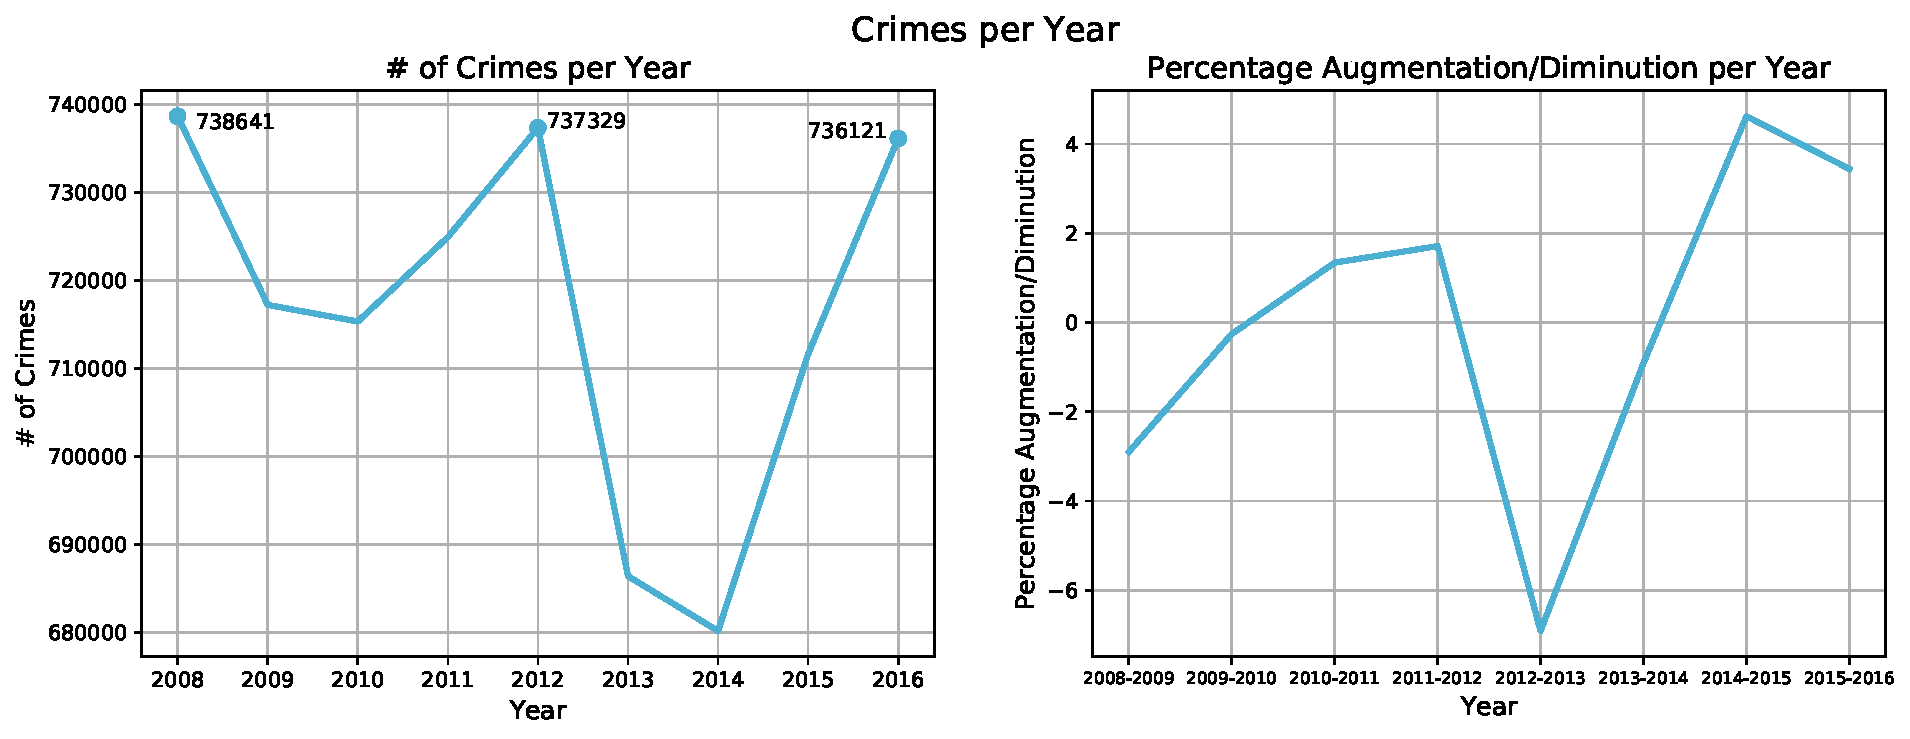
\includegraphics{../imgs/data_understanding/crimes_per_year.pdf}
                }
            \end{figure}
        \end{frame}

        \begin{frame}{Crimes per Month}
            \begin{figure}
                \centering
                \resizebox{\textwidth}{!}{
                    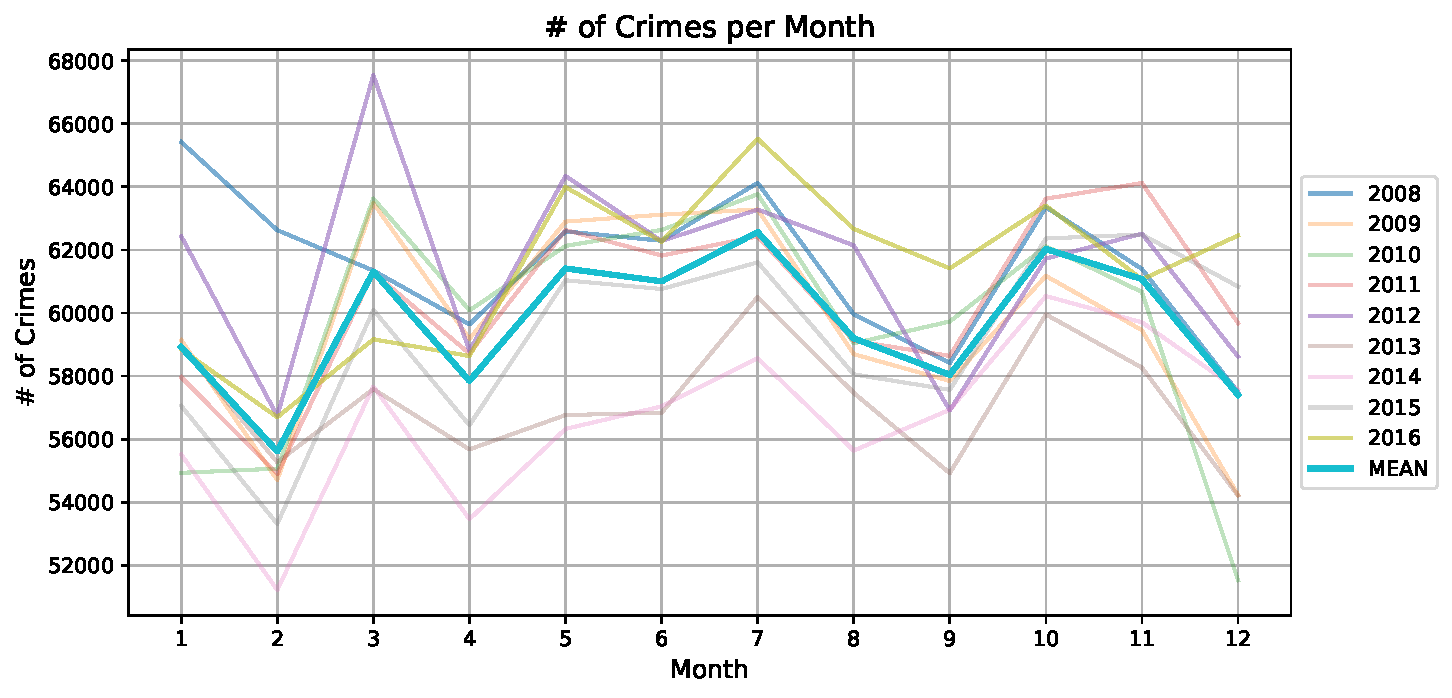
\includegraphics{../imgs/data_understanding/crimes_per_month.pdf}
                }
            \end{figure}
        \end{frame}

        \begin{frame}{Most Dangerous Years}
            \begin{figure}
                \centering
                \resizebox{\textwidth}{!}{
                    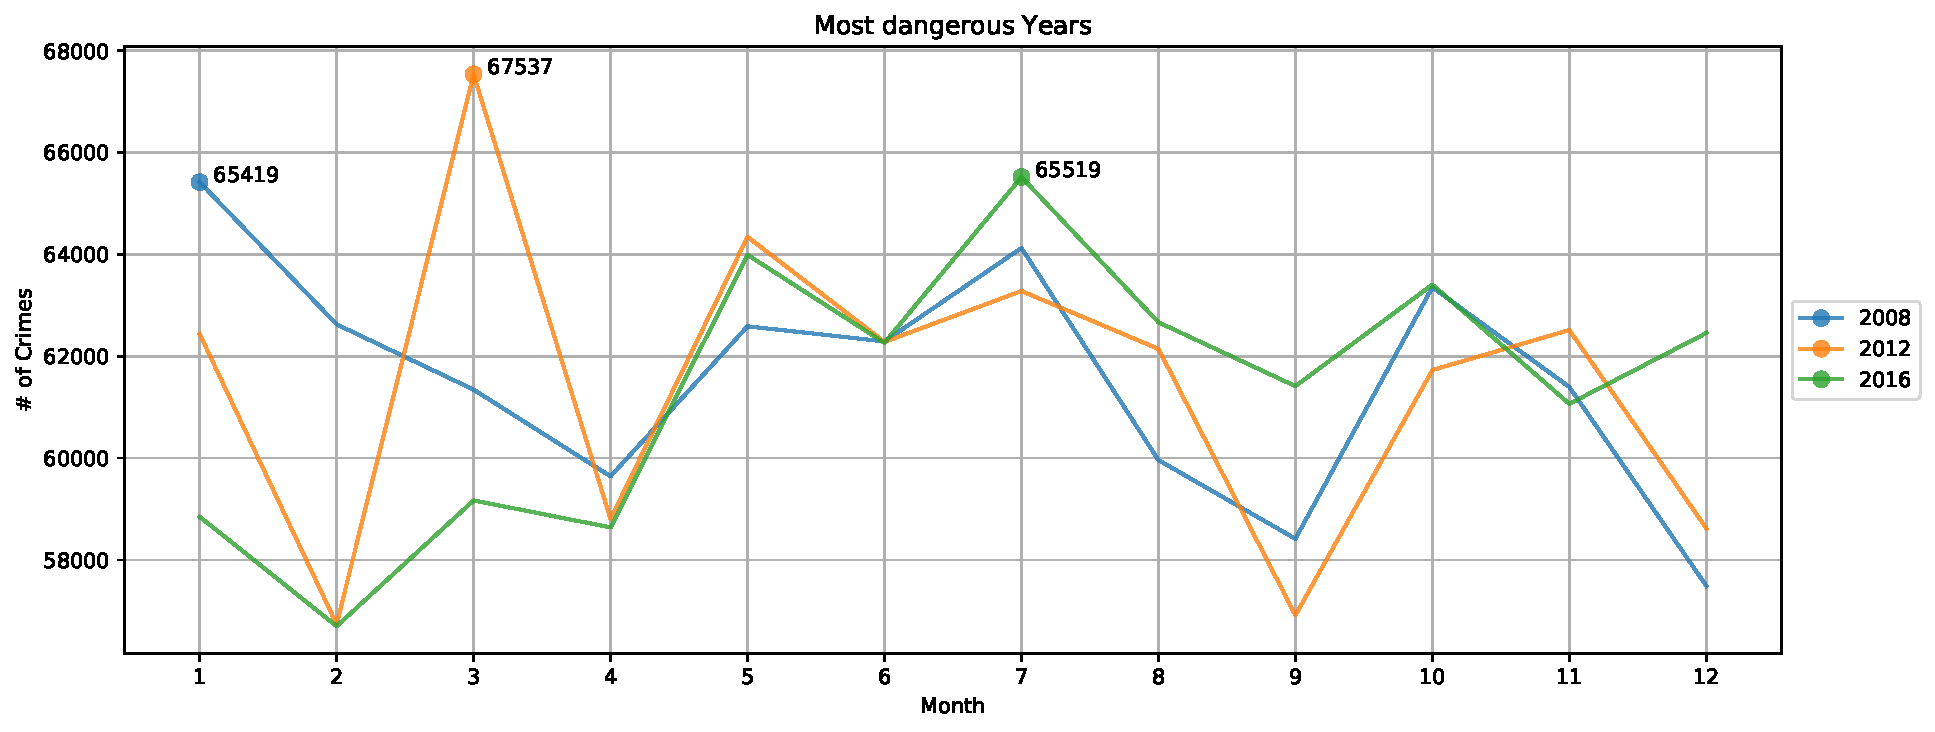
\includegraphics{../imgs/data_understanding/most_dangerous_years.pdf}
                }
            \end{figure}
        \end{frame}

        \begin{frame}{Categorical Variables' Analysis}
            \begin{itemize}
                %\item lsoa\_code has 4835 unique values, of which E01004734 is the most frequent, appearing
                %in the 0.070\% of the cropped dataset's records;
                \item \textbf{borough} has 33 unique values, of which Lambeth is the most frequent,
                appearing in the 4.47\% of the cropped dataset's records;
                \item \textbf{major\_category} has 9 unique values, of which Theft and Handling is the most
                frequent, appearing in the 33.25\% of the cropped dataset's records;
                %\item minor\_category has 32 unique values, of which Other Theft is the most frequent,
                %appearing in the 8.70\% of the cropped dataset's records;
                \item \textbf{year} has 9 unique values, of which 2016 is the most frequent, appearing in
                the 11.45\% of the cropped dataset's records;
                \item \textbf{month} has 12 unique values, of which 7 is the most frequent, appearing in the
                8.66\% of the cropped dataset's records;
            \end{itemize}
        \end{frame}

        \begin{frame}{Crimes per Borough}
            \begin{figure}
                \centering
                \resizebox{\textwidth}{!}{
                    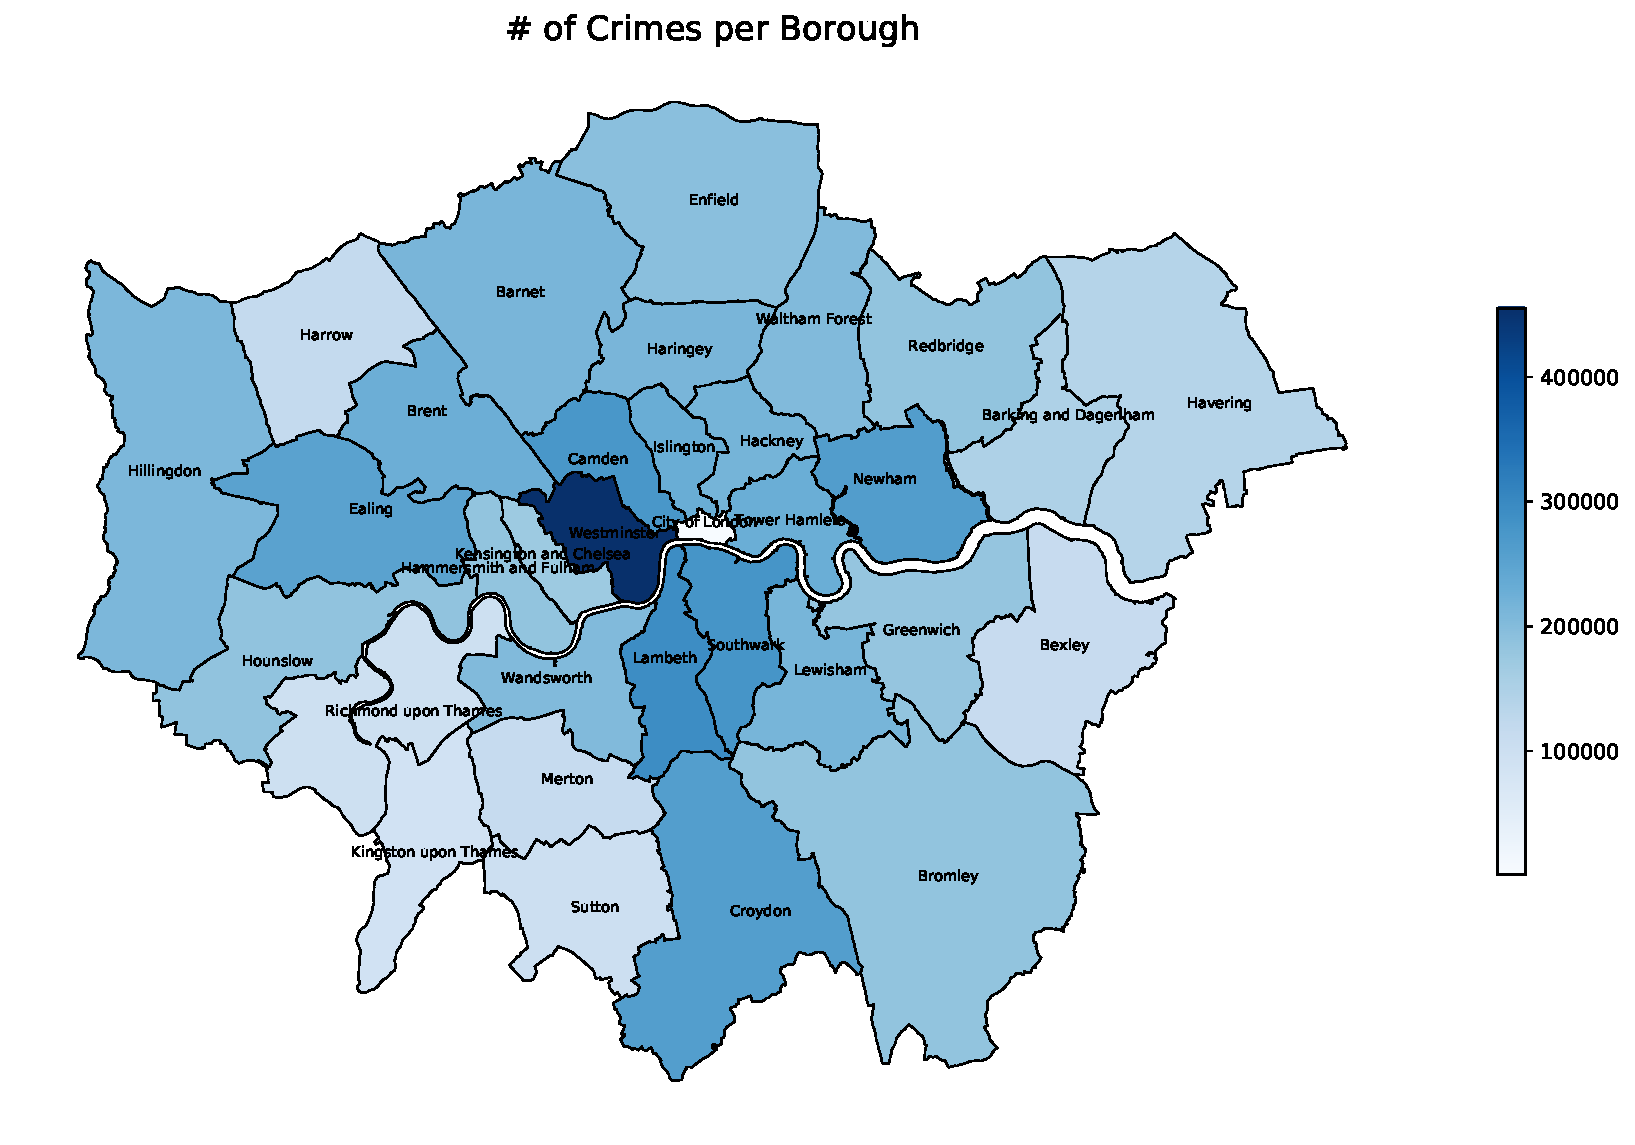
\includegraphics{../imgs/data_understanding/crimes_by_borough.pdf}
                }
            \end{figure}
        \end{frame}

        \begin{frame}{Crimes per Borough over Population Density}
            \begin{figure}
                \centering
                \resizebox{\textwidth}{!}{
                    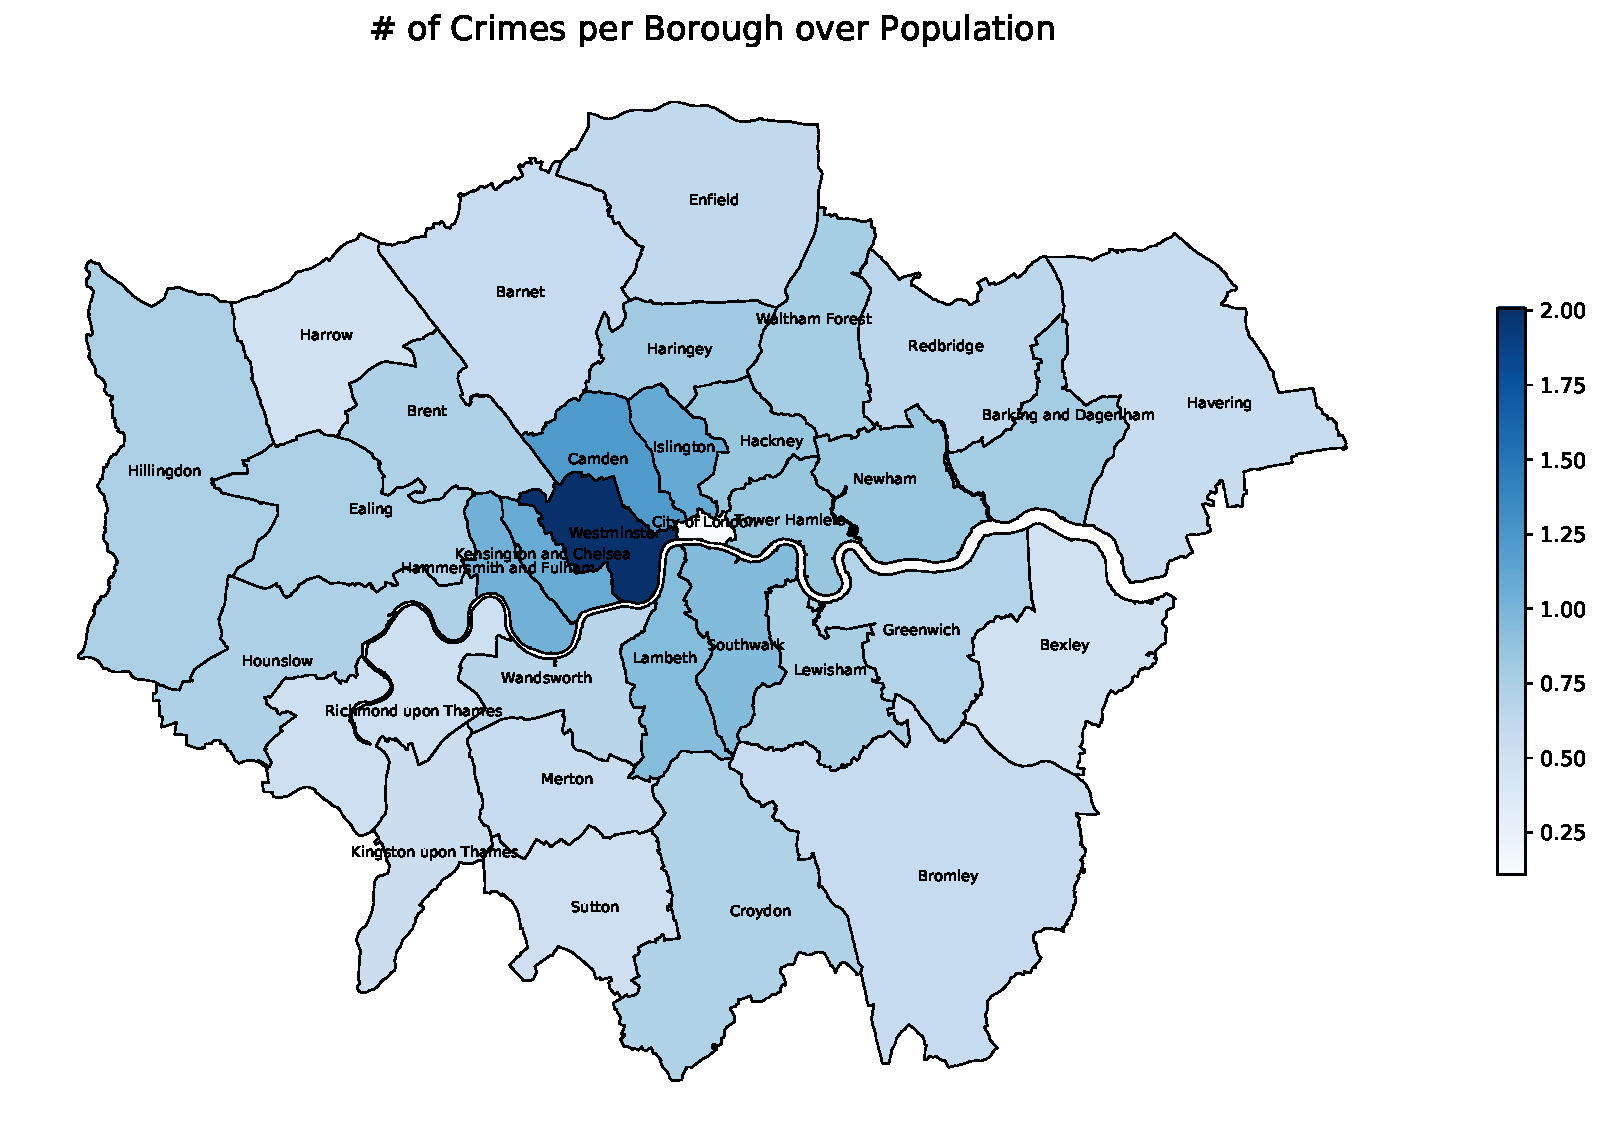
\includegraphics{../imgs/data_understanding/crimes_by_borough_over_pop.pdf}
                }
            \end{figure}
        \end{frame}

        \begin{frame}{Crimes per Major Category}
            \begin{figure}
                \centering
                \resizebox{\textwidth}{!}{
                    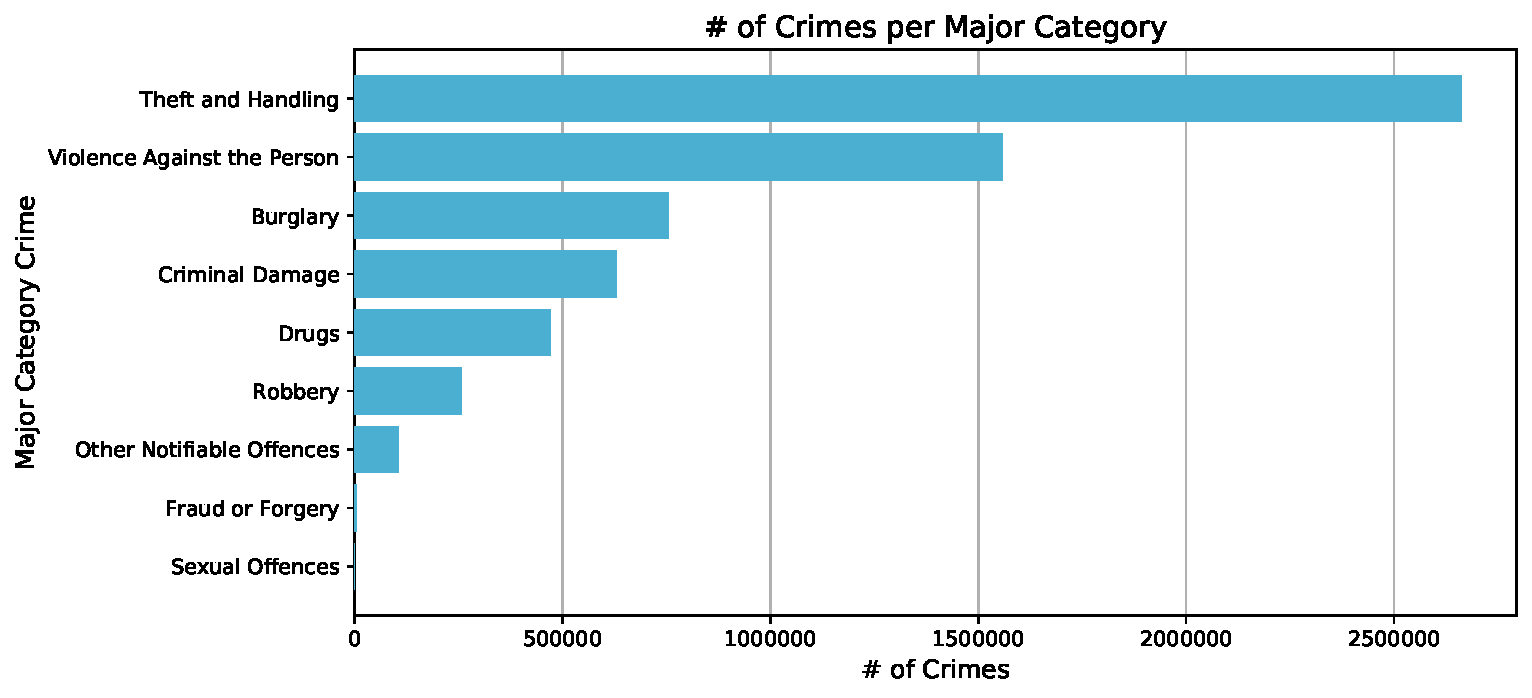
\includegraphics{../imgs/data_understanding/crimes_by_borough_major.pdf}
                }
            \end{figure}
        \end{frame}

        \begin{frame}{Major Category Crimes per Year}
            \begin{figure}
                \centering
                \resizebox{\textwidth}{!}{
                    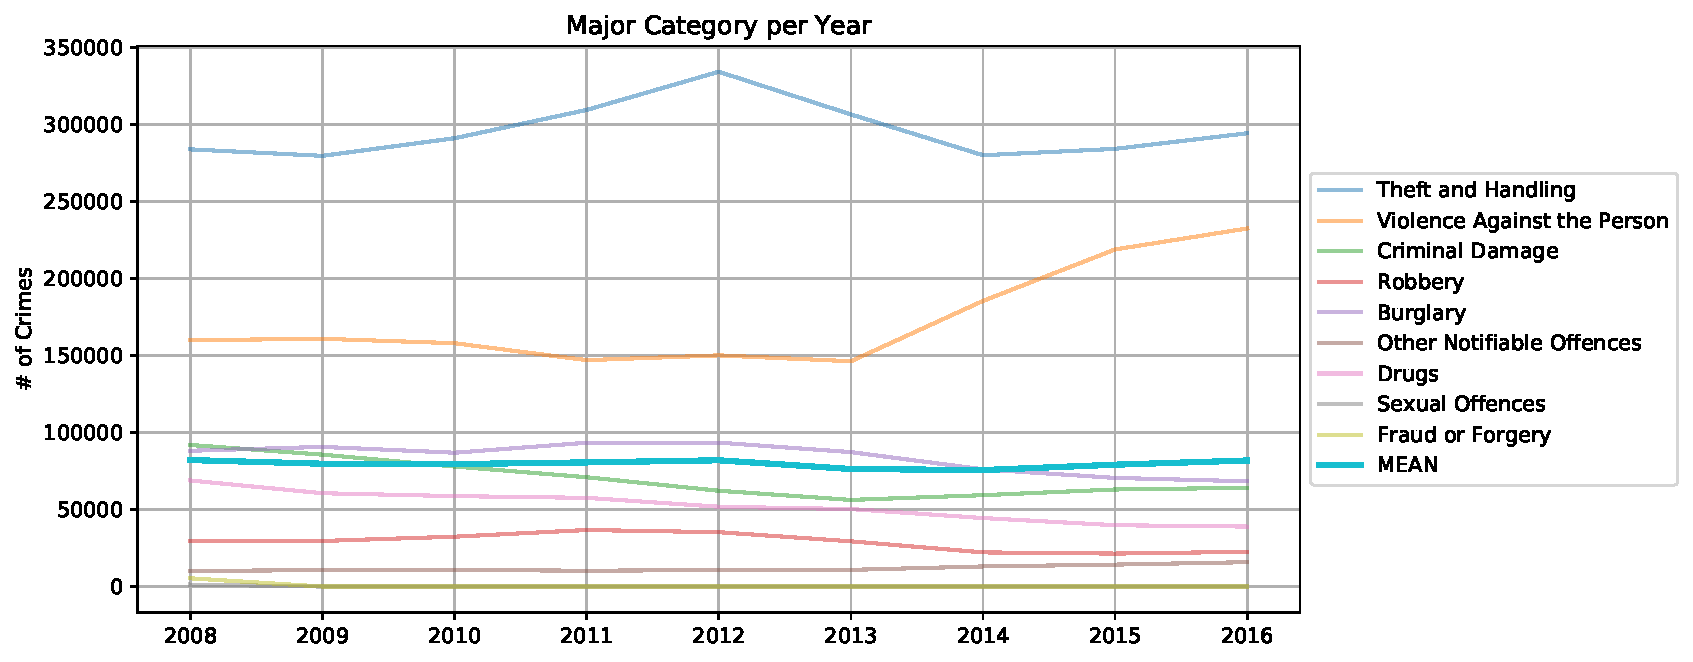
\includegraphics{../imgs/data_understanding/major_category_per_year.pdf}
                }
            \end{figure}
        \end{frame}

        \begin{frame}{Correlation Analysis}
            \begin{figure}
                \centering
                \resizebox{\textwidth}{!}{
                    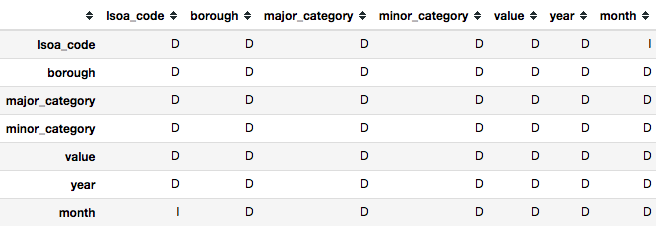
\includegraphics{../imgs/data_understanding/correlation_analysis.png}
                }
            \end{figure}
        \end{frame}
    % section data_understanding (end)

    \section{Cluster Analysis} % (fold)
    \label{sec:cluster_analysis}
        \begin{frame}{Introduction}
            I have decided to enrich the informations provided with the data understaning by searching for
            possible \textbf{cluster-like structures} in the \textbf{time series} extracted from the main
            dataset, that is, hoping to discover the similarities (or dissimilarities) among the series
            describing the criminal activities from 2008 to 2016.
        \end{frame}

        \begin{frame}{Choice of the Algorithms}
            I have used three popular clustering algorithms, that is, the \textbf{KMeans algorithm}, the
            \textbf{Hierarchical Agglomerative algorithm} and the \textbf{DBSCAN}. The three algorithms were
            adapted depending on the different series they were applied on.
        \end{frame}

        \begin{frame}{By-Year Series: Hierarchical Agglomerative Clustering}
            \begin{figure}
                \centering
                \resizebox{\textwidth}{!}{
                    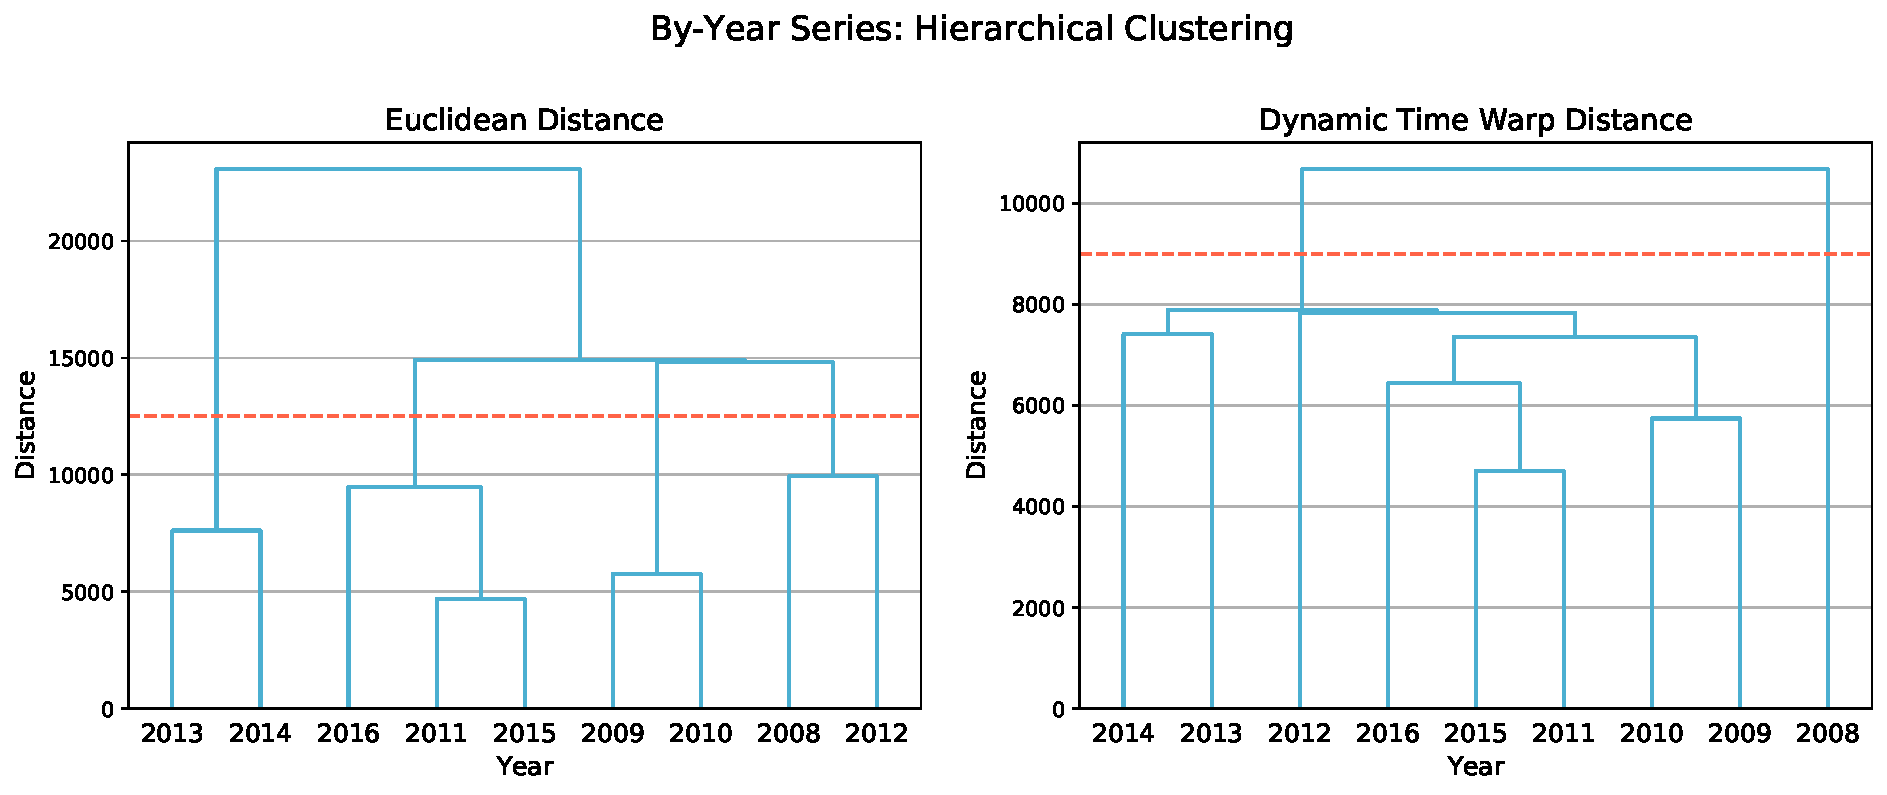
\includegraphics{../imgs/clustering/by_year_hierarchical.pdf}
                }
            \end{figure}
        \end{frame}

        \begin{frame}{By-Year Series: KMeans Algorithm and DBSCAN Clustering}
            \begin{figure}
                \centering
                \begin{subfigure}{0.20\textwidth}
                    \resizebox{\textwidth}{!}{
                        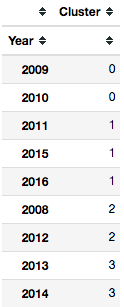
\includegraphics{../imgs/clustering/by_year_kmeans.png}
                    }
                    \caption{KMeans}
                \end{subfigure}
                \begin{subfigure}{0.20\textwidth}
                    \resizebox{\textwidth}{!}{
                        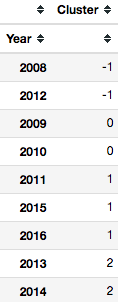
\includegraphics{../imgs/clustering/by_year_dbscan.png}
                    }
                    \caption{DBSCAN}
                \end{subfigure}
            \end{figure}
        \end{frame}

        \begin{frame}{By-Year Series: Conclusions}
            \begin{itemize}
                \item the series representing years 2013 and 2014 are the least dense of criminal
                activities, hence are clustered together;
                \item the series representing years 2008 and 2012 are the most dense of criminal activities,
                hence are clustered together;
                \item the remaining series are splitted into two distinct clusters;
            \end{itemize}
        \end{frame}

        \begin{frame}{By-Borough Series: Hierarchical Agglomerative Clustering}
            \begin{figure}
                \centering
                \resizebox{0.5\textwidth}{!}{
                    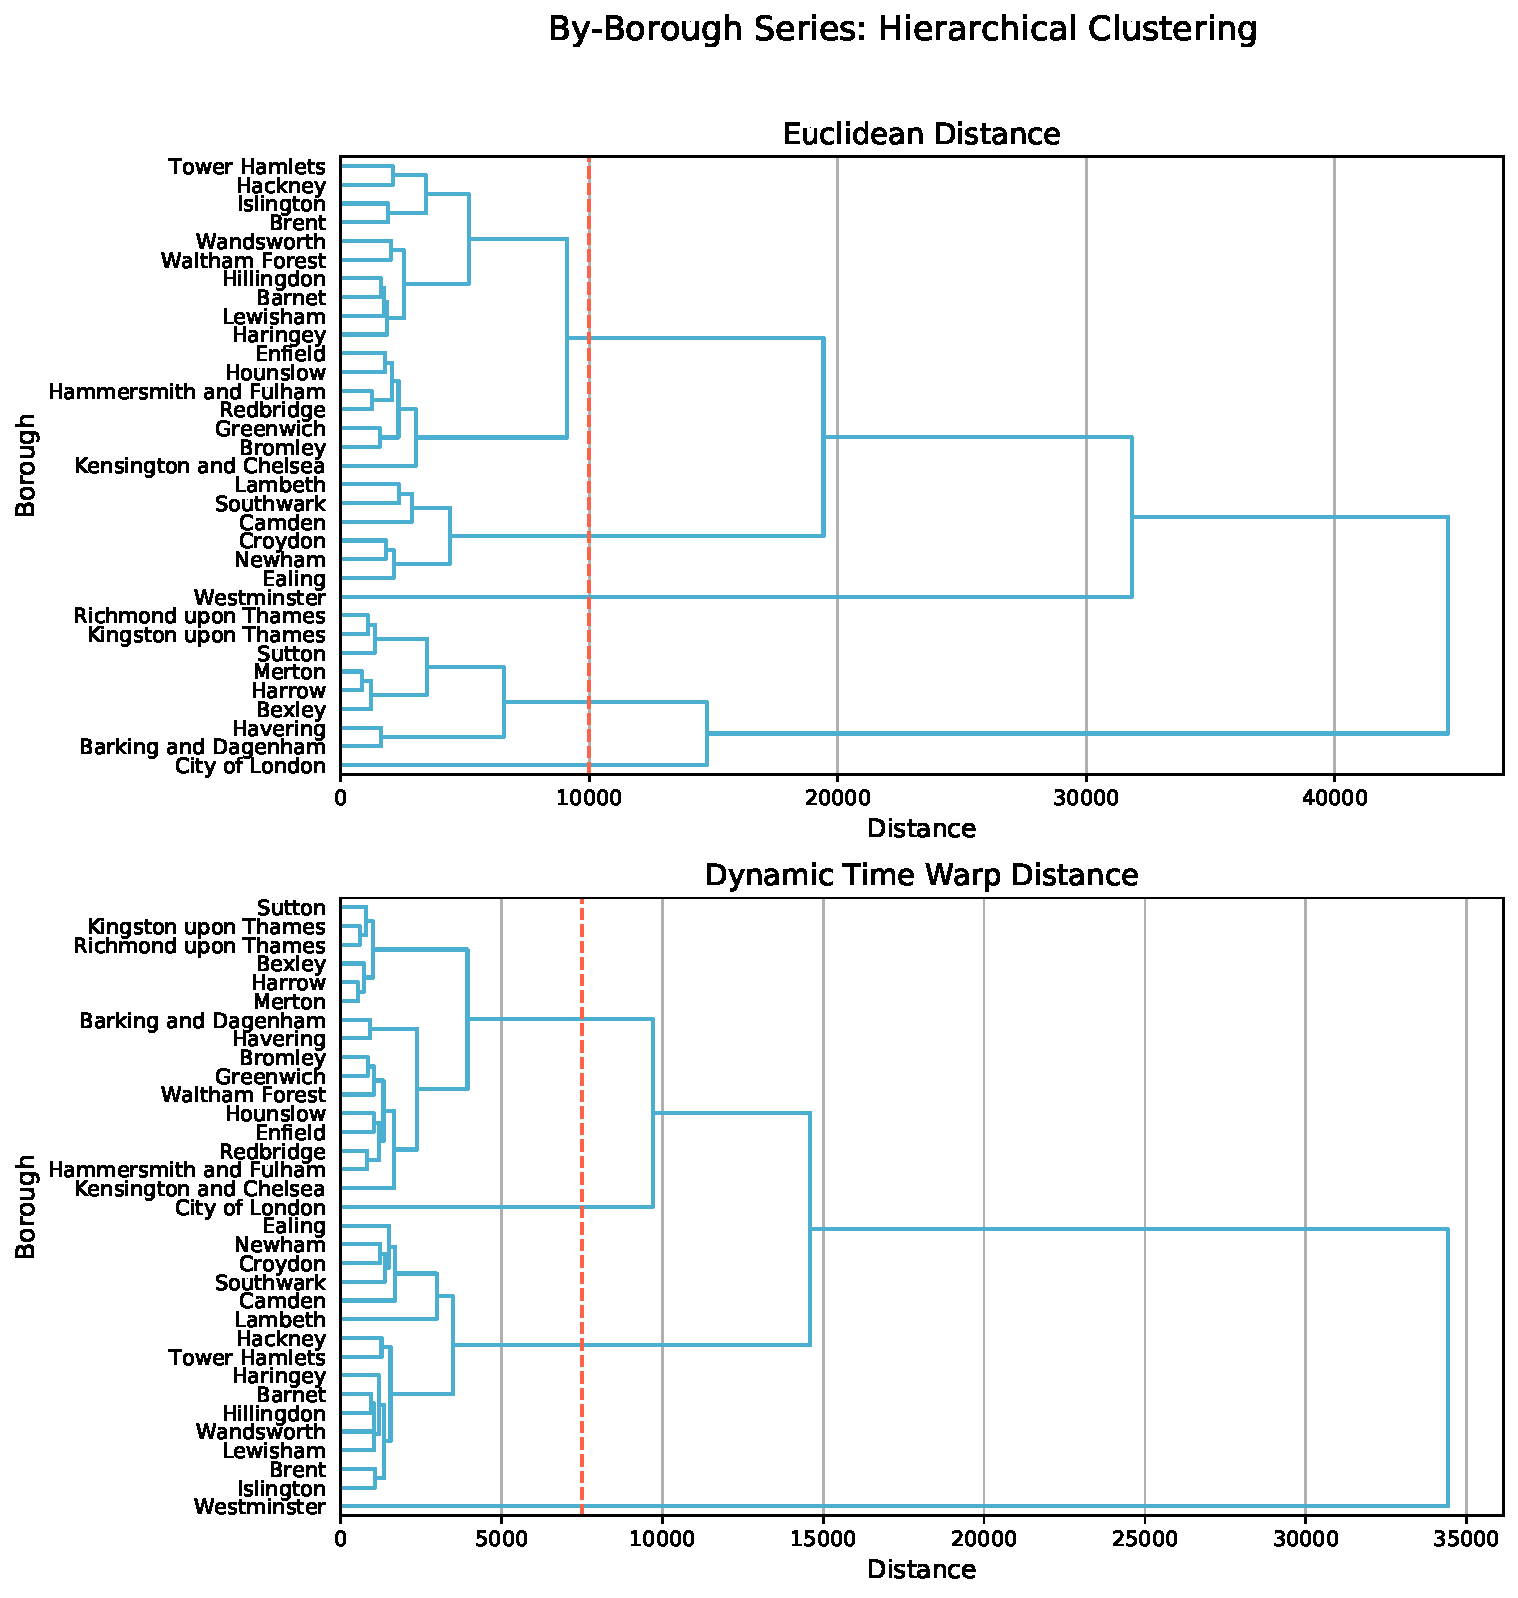
\includegraphics{../imgs/clustering/by_borough_hierarchical.pdf}
                }
            \end{figure}
        \end{frame}

        \begin{frame}{By-Borough Series: Conclusions}

        \end{frame}

        \begin{frame}{By-Major Category Series: Hierarchical Agglomerative Clustering}
            \begin{figure}
                \centering
                \resizebox{0.7\textwidth}{!}{
                    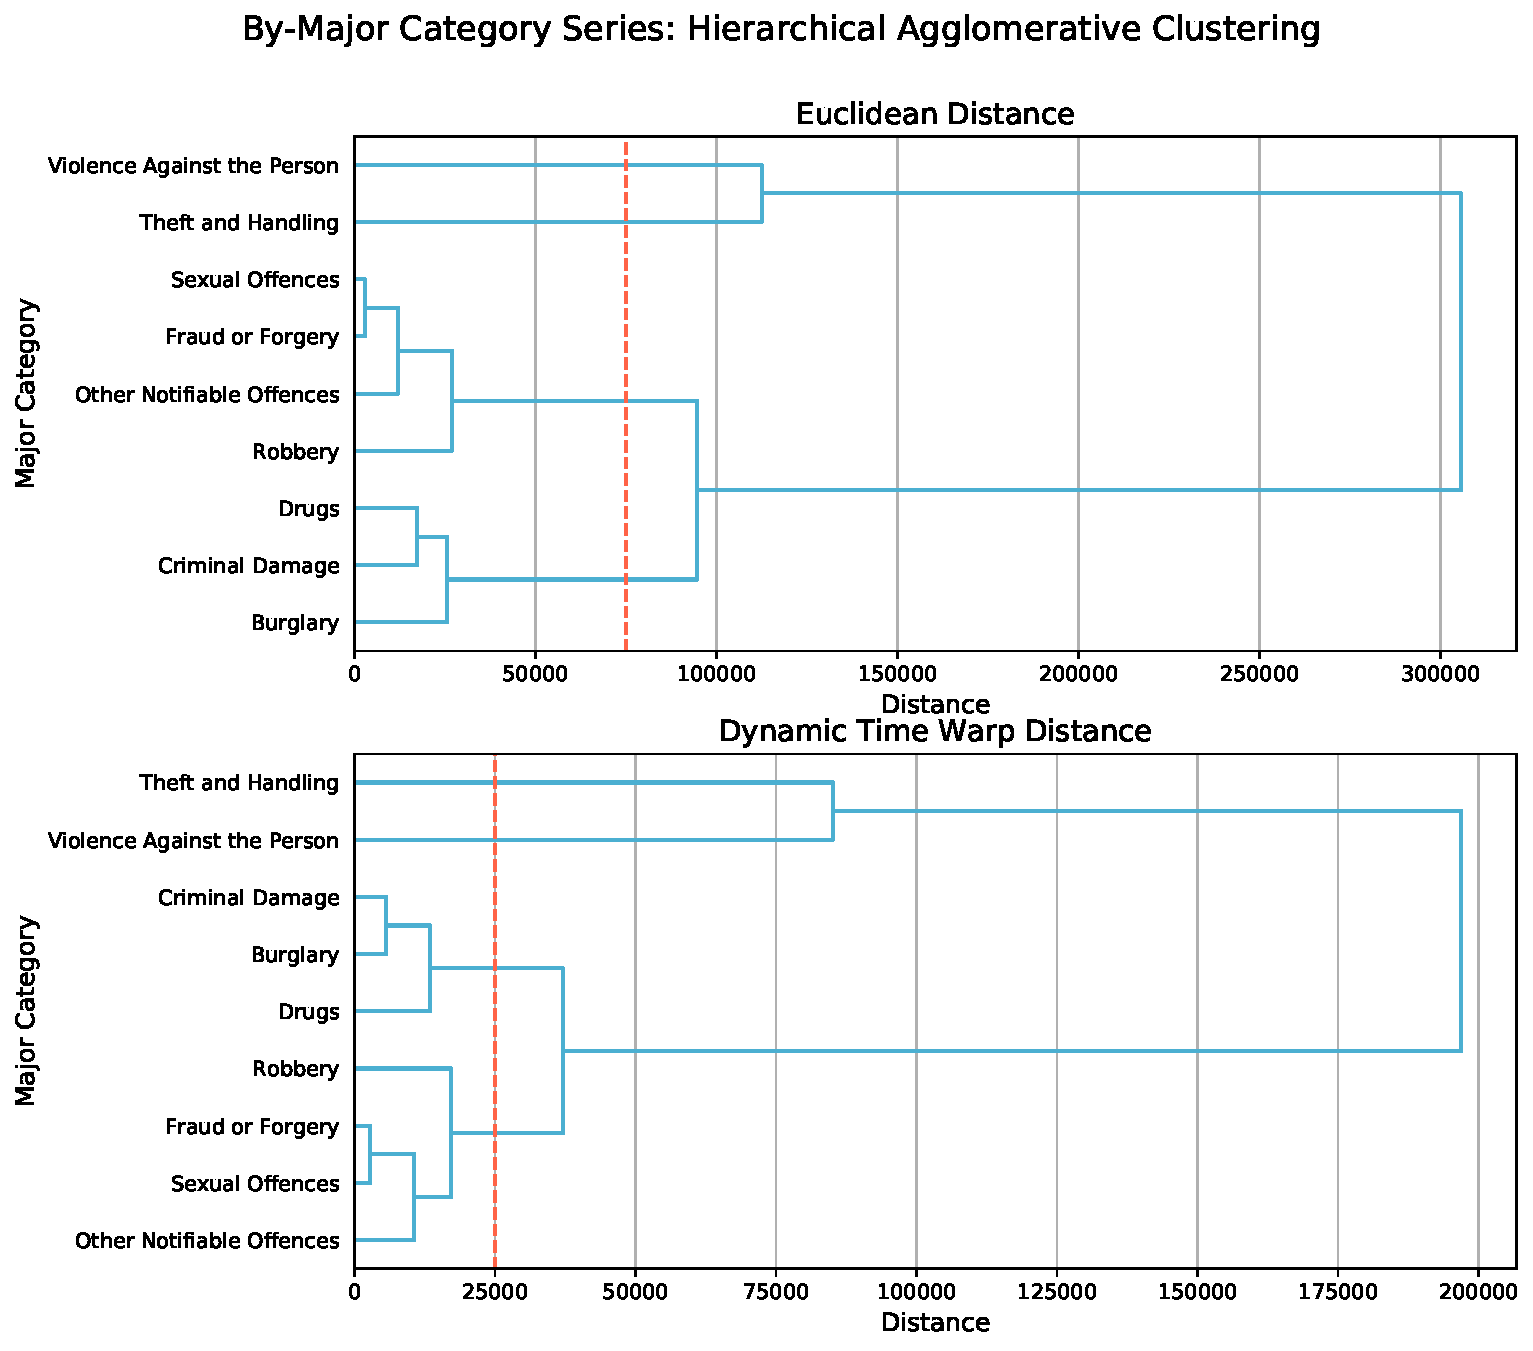
\includegraphics{../imgs/clustering/by_major_category_hierarchical.pdf}
                }
            \end{figure}
        \end{frame}

        \begin{frame}{By-Major Category Series: KMeans Algorithm and DBSCAN Clustering}
            \begin{figure}
                \centering
                \begin{subfigure}{0.30\textwidth}
                    \resizebox{\textwidth}{!}{
                        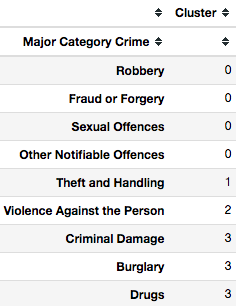
\includegraphics{../imgs/clustering/by_major_category_kmeans.png}
                    }
                    \caption{KMeans}
                \end{subfigure}
                \begin{subfigure}{0.30\textwidth}
                    \resizebox{\textwidth}{!}{
                        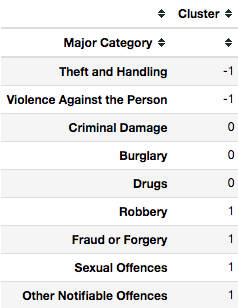
\includegraphics{../imgs/clustering/by_major_category_dbscan.png}
                    }
                    \caption{DBSCAN}
                \end{subfigure}
            \end{figure}
        \end{frame}

        \begin{frame}{By-Major Category Series: Conclusions}
            \begin{itemize}
                \item Fraud or Forgery, Sexual Offences, Other Notifiable Offences and Robbery are the least
                popular types of crimes, hence their series are clustered together;
                \item Theft and Handling and Violence Against the Person are the most popular types of
                crimes, hence they form distinct clusters for themeself;
                \item the other categories are clustered together;
            \end{itemize}
        \end{frame}
    % section cluster_analysis (end)

    \section{Forecasting} % (fold)
    \label{sec:forecasting}
        \begin{frame}{The Models - Autoregressive Model of order $p$}
            Represent by the formula

            \begin{equation*}
                X_t = c + \sum_{i = 1}^{p}\varphi_iX_{t - i} + \varepsilon_t
            \end{equation*}

            where $\varphi_{1}, \ldots , \varphi_{p}$ are the parameters of the model, $c$ is a constant,
            and $\varepsilon _{t}$ is white noise.
        \end{frame}

        \begin{frame}{The Models - Autoregressive-Moving-Average Model of orders $p$ and $q$}
            Represented by the formula

            \begin{equation*}
                X_t = c + \sum_{i = 1}^{p}\varphi_iX_{t - i} + \varepsilon_t + \sum_{i = 1}^{q}\theta_i
                \varepsilon_{t - i}
            \end{equation*}

            where $p$ and $q$ are, respectively, the autoregressive terms and the moving-average terms,
            $\varphi_{1}, \ldots , \varphi_{p}$ are the parameters of the autoregressive model,
            $\theta_1, \ldots, \theta_q$ are the parameters of the moving-average model and
            $\varepsilon_t, \varepsilon_{t - 1}, \ldots$ are white noise error terms.
        \end{frame}

        \begin{frame}{The Models - Autoregressive-Integrated-Average Model of orders $p$, $q$ and $d$}
            Represented by the formula

            \begin{equation*}
                \left ( 1 - \sum_{i=1}^p\varphi_iL^i\right )(1 - L)^dX_t =
                \left ( 1 + \sum_{i = 1}^{q}\theta_iL^i \right ) \varepsilon_t
            \end{equation*}

            where $L$ is the lag operator, $\varphi_{1}, \ldots , \varphi_{p}$ are the parameters of the
            autoregressive model, $\theta_1, \ldots, \theta_q$ are the parameters of the moving-average
            model and $\varepsilon _{t}$ is white noise.
        \end{frame}

        \begin{frame}{General Comparison}

        \end{frame}
    % section forecasting (end)
\end{document}
